\chapter{Lösungsansatz der Variablen Nachbarschaftssuche}
\label{sec:ansatz}
Als Ausgangspunkt für unser Projekt setzen wir auf bereits bewährte Techniken aus anderen Bereichen der Optimierung und versuchen, diese bestmöglich für das Partition Graph Coloring Problem einzusetzen.

\section{Aufbau der Variablen Nachbarschaftssuche}
\label{sec:vns}
Bei der Variablen Nachbarschaftssuche handelt es sich um eine metaheuristische Methode, um verschiedenste Optimierungsprobleme zu lösen. Als Metaheuristik bezeichnet man dabei Algorithmen, die andere heuristische (und manchmal auch für Teilprobleme exakte) Optimierungsverfahren steuern und deren Ergebnisse sammeln und kombinieren.

Wie der Name bereits suggeriert versucht eine VNS auf Basis unterschiedlicher Nachbarschaften eine bereits bestehende, nicht optimale Lösung zu verbessern. Eine Nachbarschaft wird im Normalfall durch sogenannte \emph{Moves}, also Züge, definiert, die beschreiben, wie man von einer Lösung zu einer Nachbarlösung kommt, die hoffentlich besser als die Ursprungslösung ist. Ein solcher Zug kann z.B.\ die Auswahl eines anderen Knotens als Repräsentant eines Clusters sein. Kann eine Lösung mit Zügen aus einer Nachbarschaft nicht mehr verbessert werden, dann befindet man sich in einem \emph{lokalen Optimum}, das leider im Normalfall nicht dem globalen Optimum -- der besten möglichen Lösung -- entspricht.

Die Variable Nachbarschaftssuche setzt nun in ihrer Optimierungskomponente (\emph{Variable Neighborhood Descent}, VND) nicht nur eine sondern gleich mehrere unterschiedliche Nachbarschaften hintereinander ein in der Hoffnung, dass ein lokales Optimum einer Nachbarschaft nicht zwangsläufig auch ein lokales Optimum einer anderen Nachbarschaft ist. Man setzt also darauf, dass eine Lösung, die in einer Nachbarschaft nicht mehr verbessert werden kann, in einer anderen Nachbarschaft sehr wohl noch Optimierungspotential besitzt. Diese neue Lösung kann dann vielleicht wieder mit einem Zug aus der ursprünglichen Nachbarschaft verbessert werden und so weiter.

Durchsucht man alle definierten Nachbarschaften systematisch (z.B.\ mittels \emph{Best Improvement} Strategie, d.h.\ von allen möglichen Zügen innerhalb einer Nachbarschaft wird jener gewählt, der die Lösung maximal verbessert) hintereinander und wiederholt nach besseren Lösungen, dann stoppt dieser Prozess erst dann, wenn eine Lösung gefunden wurde, die ein lokales Optimum bezüglich sämtlicher Nachbarschaften darstellt.

\begin{wrapfigure}[11]{r}{0.4\textwidth}
\vspace{-8mm}
\begin{center}
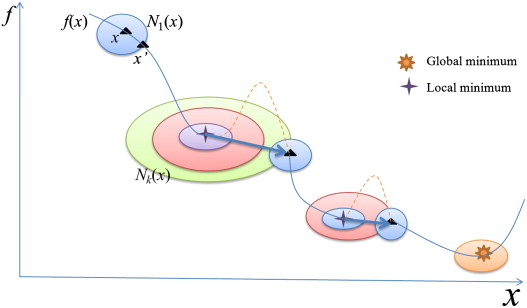
\includegraphics[width=0.4\textwidth]{../img/vns.jpg}
\end{center}
\vspace{-8mm}
\caption{Veranschaulichung der Variablen Nachbarschaftssuche. \cite{Chen}}
\vspace{-8mm}
\end{wrapfigure}

Um diesem Zustand des vollkommenen Stillstandes zu entkommen, wird, nachdem dieses lokale Optimum für alle definierten Nachbarschaften erreicht wurde, mit immer größer werdenden Kraft die Lösung ``geschüttelt''. Gemeint ist damit, dass die lokal optimale Lösung durch verschiedene Algorithmen verändert wird, welche nicht darauf abzielen, eine Lösung besser zu machen, sondern sie zunächst ein wenig, mit dem Fortschreiten der Optimierung aber auch möglichst stark zu verfremden, um einen neuen Startpunkt für das VND zu besitzen.

Veranschaulichen kann man sich das Verfahren, wenn man sich alle gültigen Lösungen als eine große Fläche vorstellt. Je nach Güte der Lösung sind einzelne Teile dieser Fläche unterschiedlich hoch, gute Lösungen bilden Senken (wenige Farben werden für die Färbung benötigt), während schlechte Lösungen Berge bilden. Das VND tendiert nun dazu, sich in einer dieser Senken festzufahren, es wurde ein lokales Optimum bezüglich sämtlicher Nachbarschaften erreicht.

Mit Hilfe des ``Schüttelns'' wird nun versucht, aus eben jenen Senken zu entkommen, um eine andere, hoffentlich tiefere Senke zu finden, also eine bessere Lösung. Nach diesem Schritt beginnt der Algorithmus nämlich wieder von vorne und sucht mit Hilfe der Nachbarschaften erneut ein lokales Optimum.

Obwohl die Variable Nachbarschaftssuche in der Theorie immer weiter laufen könnte und dabei hoffentlich immer wieder neue, bessere Lösungen erreicht, wird meist eine fixe Zeit oder eine Anzahl an Iterationen bzw.\ ``Schüttelungen'' ohne Verbesserung als Abbruchkriterium gewählt.

\begin{algorithm}
\begin{algorithmic}[1]
\State Berechne Initiallösung mit \emph{onestepCD}
\While{Terminationsbedingung \textbf{nicht} erfüllt}
\State Führe Variable Neighborhood Descent mit Best Improvement Strategie durch:
\State Nachbarschaft $l \leftarrow 1$
\While{$l \leq 3$ \textbf{und} Zeitlimit nicht erreicht}
\State Führe Nachbarschaft $n_l$ aus
\If {Lösung verbessert \textbf{und} $l\neq 1$} 
\State  $l\leftarrow 1$  
\Else
\State  $l\leftarrow l + 1$
\EndIf
\EndWhile
\If{Beste Lösung verbessert \textbf{oder} $k \geq k_{\mathrm max}$}
\State $k \leftarrow k_{\mathrm start}$ 
\Else
\State $k \leftarrow k + 1$
\EndIf
\State Wähle zufällig Nachbarschaft aus und ``schüttle" Lösung mit $k$ zufälligen Zügen
\EndWhile
\State\Return Beste gefundene Lösung
\end{algorithmic}
\caption{Pseudocode der Variablen Nachbarschaftssuche}
\end{algorithm}

\section{Konstruktionsheuristiken}
\label{sec:construct}
\citet*{Li2000} beschreiben mehrere schnelle Greedy Algorithmen zur näherungsweisen Lösung des Problems. Im Vergleich der benötigten Farben schneidet dabei der Algorithmus \emph{onestepCD} am besten ab:
\subsection{onestepCD}
Zunächst werden in einem Vorverarbeitungsschritt alle Kanten aus dem Konfliktgraphen entfernt, die Knoten innerhalb eines Clusters miteinander verbinden (da für jede Kommunikation nur genau ein Kommunikationsweg gewählt wird, können sich Knoten eines Clusters nie gegenseitig stören, die entsprechenden Kanten sind daher für die Lösung des Problems irrelevant und können gelöscht werden). Danach wird für jeden Cluster der Knoten mit der geringsten Anzahl an bereits eingefärbten Nachbarknoten bestimmt, der Knoten mit der insgesamt kleinsten Anzahl wird ausgewählt. Gibt es hier mehrere gleichwertige Kandidaten, wird aus diesen der Knoten mit der größten Anzahl an noch nicht eingefärbten Nachbarknoten gewählt bzw. -- falls dies immer noch nicht eindeutig möglich ist -- der erste Knoten aus diesen Kandidaten. Nachdem nun ein Knoten als Repräsentant für seinen Cluster bestimmt und ihm die kleinstmögliche Farbe zugewiesen wurde, werden alle anderen Knoten, die sich im selben Cluster befinden, gelöscht. Der Prozess wird solange fortgeführt, bis die Repräsentanten aller Cluster gewählt und eingefärbt sind.
\subsection{PILOT}

\section{Nachbarschaften}
\label{sec:neigh}
Wie bereits beschrieben handelt es sich bei Nachbarschaften um einzelne Algorithmen die versuchen, eine gültige Lösung in eine andere, bessere Lösung durch eine relativ kleine Änderung umzuwandeln. Wir haben uns zunächst auf die drei Nachbarschaften \emph{changeColor}, \emph{changeNode} und \emph{DSATUR} konzentiert, wobei weitere Nachbarschaften noch zur Diskussion stehen.

Jede Nachbarschaft bietet auch eine Methode an, eine Lösung zu ``schütteln'', welche ähnlich abläuft wie die Methode zur Suche des jeweiligen lokalen Optimums, allerdings ohne die Beschränkung ausschließlich bessere Ergebnisse zurückliefern zu müssen.

\subsection{ChangeColor}
\label{sec:changecolor}
Bei dieser sehr einfachen Nachbarschaft, die von der Tabu-Suche aus \citet*{Noronha2006} inspiriert ist, wird versucht, alle Knoten umzufärben, welche mit der höchsten Farbe markiert wurden. 

Um dieses Ziel zu erreichen, werden alle Knoten, welche diese höchste Farbe besitzen, mit einer neuen zufälligen Farbe markiert. Dies führt natürlich unweigerlich zu Konflikten zwischen verbundenen Knoten im Knfliktgraph, d.h.\ zu benachbarten Knoten mit gleicher Farbe. 

Um diese Konflikte zu lösen wird ein zufälliger, im Konflikt stehender Knoten ausgewählt, um ihn mit einer passenden Farbe zu füllen. Zu beachten ist hierbei die Tatsache, das diese passende Farbe kleiner sein muss als die frühere höchste Farbe, da ja eine Verbesserung (eine Reduktion der Farbenanzahl um 1) erzielt werden soll.

Sollte sich keine passende Farbe finden, wird auch dieser im Konflikt stehende Knoten mit einer zufälligen Farbe neu eingefärbt, was im Normalfall zu weitern Konflikten führt. Es wird nun versucht, diesen gesamten Vorgang so lange zu wiederholen bis keine Konflikte mehr bestehen. 

Sollte nach einer gewissen Anzahl an Iterationen keine konfliktfreie Lösung gefunden werden, bricht \emph{ChangeColor} automatisch ab und liefert die letzte valide Lösung zurück.

\subsection{ChangeNode}
\label{sec:changenode}
Diese Nachbarschaft baut auf der Tatsache auf, dass man aus einem Cluster nur jeweils einen Knoten auswählen muss. Dazu werden wie bei \emph{ChangeColor} alle Knoten höchster Farbe ausgewählt und umgefärbt.

Nun wird wieder ein zufälliger Knoten aus den entstandenen Konflikten ausgewählt, welcher dann aber durch einen zufälligen Knoten aus dem selben Cluster ersetzt wird. An diesem Knoten wird dann ein neuer Einfärbeversuch unternommen, wobei die maximal zulässige Farbe natürlich wieder kleiner ist als die ursprünglich höchste Farbe.

Dieser Vorgang wird solange wiederholt bis alle Konflikte gelöst wurden oder zu viele Iterationen abgelaufen sind.

\subsection{NewVertexColoring-DSATUR}
Diese Nachbarschaft reduziert das Graph Partition Coloring Problem auf das normale Graph Coloring Problem ohne Clusterung der Knoten, indem die aktuell gewählten Repräsentanten fixiert werden und dieses so vereinfachte Problem (das allerdings immer noch NP-hart ist) wird nun mit folgendem Greedy Ansatz näherungsweise gelöst:

\begin{enumerate}
    \item Finde den (noch nicht eingefärbten) Repräsentanten mit der größten Anzahl an eingefärbten Nachbaren (engl.\ \textit{Degree Saturation}).
    \item Bei Gleichstand: Wähle den Knoten mit der größten Anzahl an nicht eingefärbten Nachbarn.
    \item Bei Gleichstand wähle den ersten Knoten in lexikographischer Abfolge.
    \item Weise dem gewählten Knoten die kleinste mögliche Farbe zu.
    \item Wiederhole, bis die Repräsentanten aller Cluster eingefärbt wurden.
\end{enumerate}

\begin{algorithm}
\begin{algorithmic}[1]
\State Lösche die aktuelle Färbung
\State Sei $t$ der ausgewählte Knoten
\State Sei $D$ die maximale Stauration
\State Sei $B$ die maximale Anzahl an nicht eingefärbten Nachbaren
\State Sei $C$ die beste Färbung
\For{$i$ = 0,\ \ldots,\ k}
\State $D \leftarrow -1$
\State $B \leftarrow -1$
\State $C \leftarrow -1$
\State $t \leftarrow $ undefiniert
\For{alle $v \in V$}
\If{Partition von $v$ ist eingefärbt}
\State Überspringe diesen Knoten
\Else
\State $c\leftarrow$ kleinstmögliche Färbung von $v$
\State $d\leftarrow$ Anzahl an eingefärbten Nachbaren von $v$ (\textit{Degree Saturation})
\If{$d < D$}
\State Überspringe diesen Knoten
\EndIf
\State $b\leftarrow$ Anzahl an nicht eingefärbten Nachbaren von $v$ ($deg(v) - d$)
\If{$d = D \wedge b \leq B$}
\State Überspringe diesen Knoten
\EndIf
\State Wähle $v$ als besten Kandidaten:
\State $D \leftarrow d$
\State $B \leftarrow b$
\State $C \leftarrow c$
\State $t \leftarrow v$
\EndIf
\EndFor
\State Färbe $t$ mit $C$.
\EndFor
\end{algorithmic}
\caption{Pseudocode der Nachbarschaft DSATUR}
\end{algorithm}
